\chapter{Photon Identification Optimization}
\section{Topological Clusters}

Photon reconstruction is performed through a method known as ``topological clustering,'' which is outlined in Section \ref{ssec:em-signatures}. In the calorimeter, energy depositions are clustered via this method, then merged into superclusters, which are ultimately the detector signature defined as the photon. The reconstructed observables of these topological clusters, or \textit{moments}, can be used to characterize them. This section will discuss the use of these topological cluster moments in photon identification to better reject background from non-prompt photons.

\noindent\textbf{Shape Information}\\
\indent The size of the topological cell is parametrized by moments in $r_i$ and $\lambda_i$, which are defined as:

\begin{equation}
    r_i = |(\vec{x_i} - \vec{c}) \times \vec{s}| \text{\hspace{2em}(radial distance to shower axis)} \\
\end{equation}
\begin{equation}
    \lambda_i = (\vec{x_i} - \vec{c}) \cdot \vec{s} \text{\hspace{2em}(longitudinal distance to shower center of gravity)} 
\end{equation}

Where $\vec{s}$ is the shower axis and $\vec{c}$ is the center of gravity. Through this parametrization, the topo-cluster can be analyzed as a spheroid, with the second moments in $r$ and $\lambda$ as the extensions. $\sqrt{\langle \lambda^2 \rangle}$ is the semi-major axis in depth (along the shower axis), $\sqrt{\langle r^2 \rangle}$ is the semi-major axis in width.

\noindent\textbf{Location Information}\\
\indent The location of the topo-cluster is calculated from the first moments of the three cartesian coordinates, describing the position of $\vec{c}$. Due to azimuthal symmetry in the detector, the key component to locational parametrization of topo-clusters is the depth in the calorimeter. Thus, this location can be described via $\lambda_{clus}$, the distance of the center of gravity from the front face of the calorimeter.

A visualization of the geometric moments, both location and shape can be found in Figure \ref{fig:topo-geom}, with relevant spacial parameters (i.e. $\vec{c}$, $\vec{s}$, etc) shown and defined.

\begin{figure}[!thp]
    \centering
    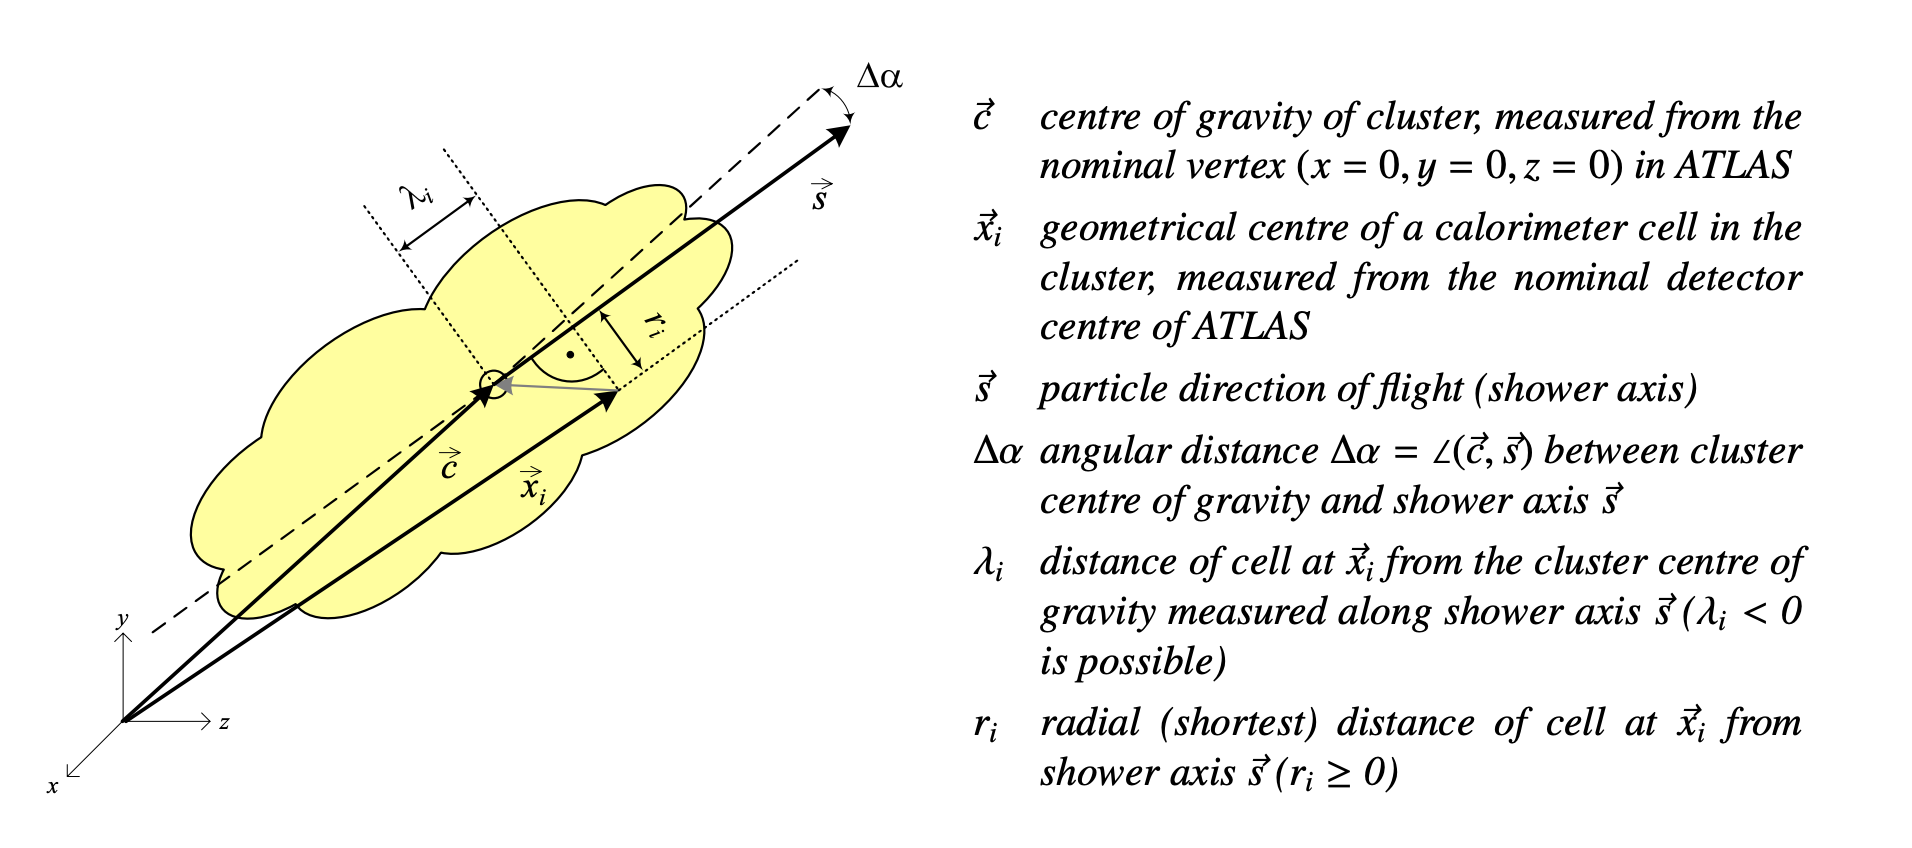
\includegraphics[width=.90\textwidth]{chapters/chapter4_photonID/images/geom-moments.png}

    \caption[The geometric moments and relevant parameters for topo-clusters.]
    {The geometric moments and relevant parameters for topo-clusters \cite{topo-clustering-r1}.}
    \label{fig:topo-geom}
\end{figure}


\section{Multivariate Analysis Techniques}

The current photon identification working points are defined by a rectangular cuts method. Cut optimization is performed through a 9-dimensional scan over the shower shape variables. In order to better reject background, a multivariate approach to defining these working points has been investigated. These methods are outlined in detail in Appendix \ref{app:MVA}, and the following sections will discuss the improvements brought to photon identification through implementing them.

\subsection{Boosted Decision Tree}
\subsection{Neural Network}